%-------------------------
% Resume in Latex
% Author : Sourabh Bajaj
% License : MIT
%------------------------

\documentclass[letterpaper,11pt]{article}
\usepackage{wrapfig}
\usepackage{cutwin}
\usepackage[UTF8]{ctex}
\usepackage{latexsym}
\usepackage[empty]{fullpage}
\usepackage{titlesec}
\usepackage{marvosym}
\usepackage[usenames,dvipsnames]{color}
\usepackage{verbatim}
\usepackage{enumitem}
\usepackage{hyperref}
\usepackage{fancyhdr}
\usepackage{graphicx}
\usepackage{subfigure}
\usepackage{amsmath,boxedminipage}
\usepackage{setspace}
\pagestyle{fancy}
\fancyhf{} % clear all header and footer fields
\fancyfoot{}
\renewcommand{\headrulewidth}{0pt}
\renewcommand{\footrulewidth}{0pt}

% Adjust margins
% \usepackage{geometry}
% \geometry{a4paper}
% \geometry{left=1cm,right=1cm,top=1cm,bottom=1cm}

\addtolength{\oddsidemargin}{-0.8in}
\addtolength{\evensidemargin}{0.8in}
\addtolength{\textwidth}{1.6in}
\addtolength{\topmargin}{-0.85in}
\addtolength{\textheight}{1.7in}

\urlstyle{same}

\raggedbottom
\raggedright
\setlength{\tabcolsep}{0in}

% Sections formatting
\titleformat{\section}{
  \vspace{-4pt}\scshape\raggedright\large
}{}{0em}{}[\color{black}\titlerule \vspace{-5pt}]

% \hypersetup{
% colorlinks=true,
% linkcolor=black
% }
\hypersetup{
    colorlinks=false,
    linkcolor=black,
    pdfborder={0 0 0}
    % filecolor=magenta,
    % urlcolor=cyan,
    % linkbordercolor=white
}
% \usepackage[hidelinks]{hyperref}
%-------------------------
% Custom commands
\newcommand{\resumeItem}[2]{
  \item\small{
    \textbf{#1}{ #2 \vspace{-2pt}}
  }
}

\newcommand{\resumeSubheading}[4]{
  \vspace{-1pt}\item
    \begin{tabular*}{0.97\textwidth}{l@{\extracolsep{\fill}}r}
      \textbf{#1} & #2 \\
      \textit{\small#3} & \textit{\small #4} \\
    \end{tabular*}\vspace{-5pt}
}

\newcommand{\resumeSubItem}[2]{\resumeItem{#1}{#2}\vspace{-4pt}}

\renewcommand{\labelitemii}{$\circ$}

\newcommand{\resumeSubHeadingListStart}{\begin{itemize}[leftmargin=*]}
\newcommand{\resumeSubHeadingListEnd}{\end{itemize}}
\newcommand{\resumeItemListStart}{\begin{itemize}}
\newcommand{\resumeItemListEnd}{\end{itemize}\vspace{-5pt}}

%-------------------------------------------
%%%%%%  CV STARTS HERE  %%%%%%%%%%%%%%%%%%%%%%%%%%%%


\begin{document}
\begin{spacing}{0.9}
 %----------HEADING-----------------
\begin{wrapfigure}[0]{r}{70pt}
\vspace{-35pt}
\begin{boxedminipage}{78pt}
\centering
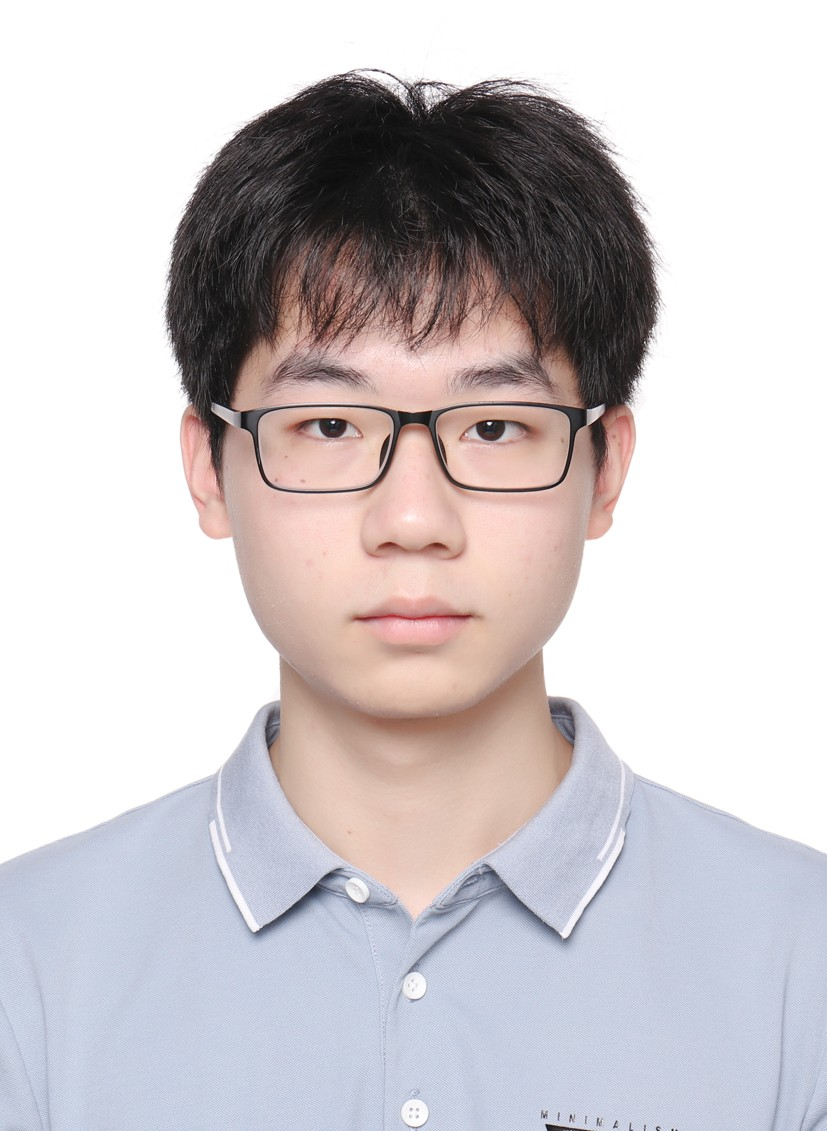
\includegraphics[width=60pt]{me.jpg}
\end{boxedminipage}
\end{wrapfigure}

\begin{tabular*}{0.3\textwidth}{l@{\extracolsep{\fill}}r}
  \textbf{{\huge 孔昊}} \\
    中国, 南京, 江宁区, 将军大道29号, 	211106 \\
    电话:  +86\ 18901972939 \\
    邮箱: \href{mailto:andy.kong@nuaa.edu.cn}{andy.kong@nuaa.edu.cn} \\
    GitHub: \href{https://github.com/AndyKong2020}{github.com/AndyKong2020} \\
\end{tabular*}
\vspace{-0.5em}
%-----------EDUCATION-----------------
\section{教育背景}
  \resumeSubHeadingListStart
    \resumeSubheading
      {南京航空航天大学自动化学院}{南京}
      {修读专业: 自动化}{2021.09 - 至今}
      \resumeItemListStart
        \resumeItem{GPA:}{2.9} 
        \resumeItem{相关课程:}{C语言程序设计, 计算机软件技术基础, 自动控制原理, 嵌入式测控系统, 人工智能概论, 计算机视觉和人工智能}
      \resumeItemListEnd
  \resumeSubHeadingListEnd
  \vspace{-1em}
  
\section{项目和经历}
  \resumeSubHeadingListStart
    \resumeSubheading
      {算法组, \href{https://github.com/nuaa-rm}{南京航空航天大学RoboMaster长空御风战队}}{南京、常州、深圳}
      {2023赛季算法组成员,2025赛季算法组项目负责人}{2021.12 - 至今}
      \resumeItemListStart
        \resumeItem{核心项目:}
          {为机器人开发自动瞄准及自动开火算法,使用pnp进行位姿估计,基于IMM、KF和EKF的状态预测,基于目标运动学建模的自动开火控制,实现高性能,高可靠性,模块间松耦合,赛场表现在一众强队中处于领先水平。}
        \resumeItem{}
          {入队培训期间开发了\href{https://github.com/AndyKong2020/rm_benchmark}{视觉识别算法的benchmark工具},\href{https://github.com/AndyKong2020/Bilibili-Spidar}{爬取比赛对手录像工具}等项目。}
        \resumeItem{}
          {参与开发比赛机器人操作ui界面的\href{https://ui.bismarck.xyz/}{图形化开发工具},使用前端技术栈。}
        \resumeItem{项目管理:}
          {全流程主导人员培训、选拔、考核。协调10人团队,负责目标拆解、模块解耦、技术方案制定、研发进度管理以及资源调配工作,实现了精确的目标管理。推动基于GitHub的版本管理和协作流程以及okr管理,制定可量化的测试标准,确保团队高效运作。}
      \resumeItemListEnd
    \resumeSubheading
      {\href{https://res.nuedc-training.com.cn/topic/2023/topic_101.html}{全国大学生电子设计竞赛飞行器选题}}{南京}
      {队长, 组织者, 算法}{2023.06 - 2023.08}
      \resumeItemListStart
      \resumeItem{}
        {基于ROS1开发\href{https://github.com/AndyKong2020/RubicJellyfish}{无人机全套任务执行方案},承担软件的架构设计和接口设计。}
      \resumeItem{}
        {完成题目要求包括路径巡航、自主搜寻、目标识别、物品投放、地空协同等在内的所有任务,基于单例和异步设计的任务调度器。}
      \resumeItem{}
        {进度管理,跨学科协调队内机械、电控高效率合作。}
      \resumeItemListEnd
    \resumeSubheading
      {中国机器人大赛先进视觉项目}{常州、泉州}
      {团队成员}{2022.08 - 2022.12}
      \resumeItemListStart
        \resumeItem{}
          {负责工业测量项目算法开发,使用点云数据pca进行参数测量,基于ROS1和PCL库开发,测量精度显著提升。}
         \resumeItem{}
          {YOLOV5、V7的数据集标注、模型训练、部署经历,不同平台复杂环境配置经历。}
      \resumeItemListEnd
    % \resumeSubheading
      % {南京航空航天大学电子电路设计竞赛}{南京}
      % {队长, 组织者, 算法}{2022.11}
      % \resumeItemListStart
      %   \resumeItem{}
      %     {基于ROS的分布式架构小车,实现远端神经网络推理运算。}
      % \resumeItemListEnd
    % \resumeSubheading
    %   {南京航空航天大学航模队}{南京}
    %   {队员}{2021.11 - 至今}
    %   \resumeItemListStart
    %     \resumeItem{}
    %       {参与航模队培训,学习飞控原理及固定翼飞机结构设计}
    %     \resumeItem{}
    %       {飞控调参,各类穿越机、旋翼无人机、固定翼无人机驾驶经验}
    %   \resumeItemListEnd
%   \resumeSubHeadingListEnd
  


% \section{实习}
%  \resumeSubHeadingListStart
    \resumeSubheading
      {杭州优赛机器人有限公司}{杭州}
      {实习,算法岗}{2024.10 - 2024.12}
      \resumeItemListStart
        \resumeItem{}
          {承担德国南毛集团张家港工厂的自动清洁机器人车端上层算法开发,基于ROS的架构设计,独自完成move\_base框架下的完整demo开发与调试。}
        \resumeItem{}
          {开发机器人的路径覆盖算法,实现牛耕法和A\_Star的路径规划,实现可控的路径生成和可自定义清扫区域。}
        \resumeItem{}
          {承担面向VDA5050协议的车端-调度端接口开发,实现跨ROS和MQTT通信协议的双向通信,编写基于Python的自动化测试脚本。与调度端跨部门协作。}
        \resumeItem{}
          {为公司搭建gitlab私有代码托管服务器,推动git版本管理在项目中的使用。}
      \resumeItemListEnd
 \resumeSubHeadingListEnd
 \vspace{-1em}


 \section{获奖情况}
 \resumeSubHeadingListStart
    \resumeSubItem{国家级一等奖*2:}
    {第二十二届全国机器人大赛RoboMaster2023机甲大师超级对抗赛 全国赛 \textbf{\&} 区域赛(中部赛区),}
    {2023.08}
    % \resumeSubItem{国家级一等奖:}
    % {第二十二届全国机器人大赛RoboMaster2023机甲大师超级对抗赛 区域赛(中部赛区),}
    % {2023.08}
    \resumeSubItem{国家级一等奖:}
    {第二十二届全国机器人大赛RoboMaster2023机甲大师超级对抗赛,哨兵机器人组 机器人实战奖,}
    {2023.08}    
    \resumeSubItem{国家级二等奖:}
    {2023 年 TI 杯全国大学生电子设计竞赛,}
    {2023.09}
    \resumeSubItem{国家级二\textbf{\&}三等奖:}
    {2022中国机器人大赛暨ROBOCUP机器人世界杯中国赛,3D识别赛项 \textbf{\&} 工业测量赛项,}
    {2023.02}
    % \resumeSubItem{国家级三等奖:}
    % {2022中国机器人大赛暨ROBOCUP机器人世界杯中国赛,工业测量赛项,}
    % {2023.02}
    \resumeSubItem{省级一等奖*2:}
    {2022年 \textbf{\&} 2023年江苏省大学生电子设计竞赛,}
    {2022.09, 2023.09}
    % \resumeSubItem{省级一等奖:}
    % {2023年江苏省大学生电子设计竞赛,}
    % {2023.09}
    \resumeSubItem{省级二等奖:}
    {第二十二届全国机器人大赛RoboMaster2023机甲大师高校联盟赛 (江苏站),}
    {2023.08}
    \resumeSubItem{省级二等奖:}
    {第十三届江苏省大学生机器人大赛,}
    {2022.06}
    \resumeSubItem{省级二等奖:}
    {2022年第八届中国国际 “互联网+”大学生创新创业大赛江苏省选拔赛,}
    {2022.06}
    \resumeSubItem{校级特等奖\textbf{\&}一等奖:}
    {第十六届 \textbf{\&} 第十七届南京航空航天大学电子电路设计竞赛,}
    {2021.12, 2023.02}
    
 \resumeSubHeadingListEnd
 \vspace{-0.8em}
%--------PROGRAMMING SKILLS------------
\section{语言和技能}
 \resumeSubHeadingListStart
 \resumeSubItem{语言能力:}{IELTS 7}
 \resumeSubItem{主要编程语言和技术栈:}{C++, ROS, Linux, Git, Python \\}
 \begin{spacing}{0.3}
 \end{spacing}
 \resumeSubItem{技能:}{熟悉ROS框架的项目开发,熟悉ROS项目的测试与调试,熟练使用Linux系统;\\
     熟悉机器视觉原理及编程实践,擅长建模解决具体问题,擅长跨部门沟通协作及程序优化;\\
     熟练使用现代主流开发工具链及版本管理工具,有良好的团队协作能力,有丰富的项目管理经验;\\
     有较强的自学能力,能够快速学习新技术。有较广的技术栈,能够理解其他技术团队的工作并针对性优化自己的工作。有较强的抗压能力,能够在高强度的工作环境下保持高效率工作。}
 \resumeSubHeadingListEnd
 
\end{spacing}
% \end{document}



% \begin{document}
\begin{spacing}{1.3}
%----------HEADING-----------------
\begin{wrapfigure}[0]{r}{70pt}
\vspace{-35pt}
\begin{boxedminipage}{78pt}
\centering
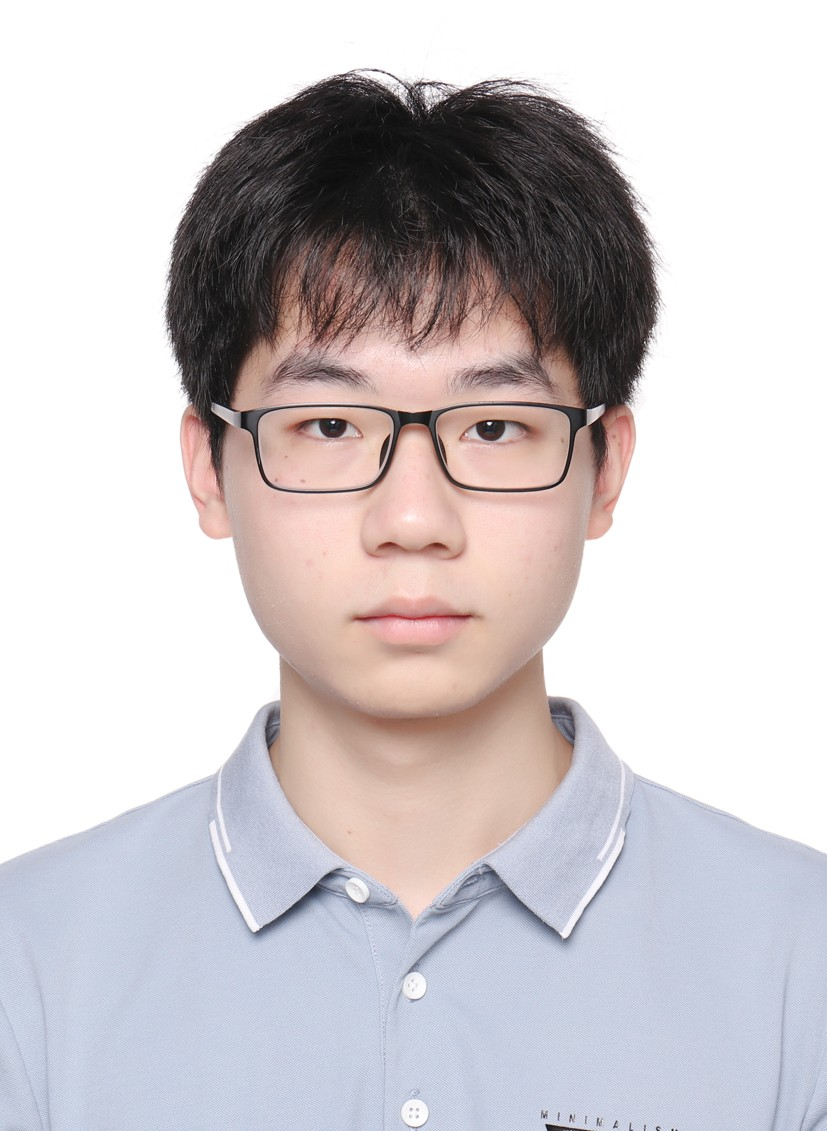
\includegraphics[width=65pt]{me.jpg}
\end{boxedminipage}
\end{wrapfigure}

\begin{tabular*}{0.3\textwidth}{l@{\extracolsep{\fill}}r}
 \vspace{-2pt} \\
  
  \textbf{{\huge Hao Kong}} \\
    Jiangning District, Nanjing, China, 29 Jiangjun Avenue, 211106 \\
    Phone: +86\ 18901972939 \\
    Email: \href{mailto:andy.kong@nuaa.edu.cn}{andy.kong@nuaa.edu.cn} \\
    GitHub: \href{https://github.com/AndyKong2020}{github.com/AndyKong2020} \\
\end{tabular*}
% \vspace{-0.5em}
%-----------EDUCATION-----------------
\section{Education}
  \resumeSubHeadingListStart
    \resumeSubheading
      {College of Automation Engineering, Nanjing University of Aeronautics and Astronautics}{Nanjing, China}
      {Major: Automation Engineering}{Sep. 2021 - Present}
      \resumeItemListStart
        \resumeItem{GPA:}{2.9} 
        \resumeItem{Relevant Courses:}{C Programming, Basic Computer Software Technology, Automatic Control Principle, Embedded Testing and Control Systems, Introduction to Artificial Intelligence, Computer Vision and Artificial Intelligence}
      \resumeItemListEnd
  \resumeSubHeadingListEnd
  % \vspace{-1em}

%-----------PROJECTS AND EXPERIENCE-----------
\section{Projects and Experience}
  \resumeSubHeadingListStart
    \resumeSubheading
      {Algorithm Team, \href{https://github.com/nuaa-rm}{RoboMaster Competition, Team CKYF, NUAA}}{Nanjing, Changzhou, Shenzhen}
      {Algorithm Team Member (2022-2023), Project Leader (2024-2025)}{Dec. 2021 - Present}
      \resumeItemListStart
        \resumeItem{Core Projects:}
          {Developed automatic aiming and firing algorithms for robots, using PnP for pose estimation, IMM, KF, and EKF for state prediction, and motion modeling for automatic firing control. Achieved high performance, reliability, and modular loose coupling, leading to superior competition results.}
        \resumeItem{}
          {During training, developed tools such as \href{https://github.com/AndyKong2020/rm_benchmark}{a benchmark tool for visual recognition algorithms} and \href{https://github.com/AndyKong2020/Bilibili-Spidar}{a web scraper for opponents’ match videos}.}
        \resumeItem{}
          {Contributed to the development of a \href{https://ui.bismarck.xyz/}{GUI development tool} for robot operation UI using a front-end technology stack.}
        \resumeItem{Project Management:}
          {Led the entire process of personnel training, selection, and assessment. Coordinated a team of 10 members, responsible for target breakdown, module decoupling, technical solution development, R\&D progress management, and resource allocation, achieving precise goal management. Promoted GitHub-based version control and collaboration processes, as well as OKR management, and established quantifiable testing standards to ensure efficient team operation.}
      \resumeItemListEnd
    \resumeSubheading
      {\href{https://res.nuedc-training.com.cn/topic/2023/topic_101.html}{TI Cup 2023 National Undergraduate Electronic Design Competition}}{Nanjing}
      {Team Leader, Organizer, Algorithm Developer}{Jun. 2023 - Aug. 2023}
      \resumeItemListStart
        \resumeItem{}
          {Developed a complete task execution solution for \href{https://github.com/AndyKong2020/RubicJellyfish}{the ground-air collaborative system} based on ROS1, taking responsibility for software architecture design and interface design.}
        \resumeItem{}
          {Completed all tasks required by the project, including path cruising, autonomous searching, target recognition, item delivery, and ground-air coordination, using a task scheduler based on the singleton design pattern and asynchronous design.}
        \resumeItem{}
          {Managed progress and facilitated collaboration between mechanical and electronic teams to ensure efficiency.}
      \resumeItemListEnd
    \resumeSubheading
      {22nd RoboCup China Open, Advanced Vision Project}{Changzhou, Quanzhou}
      {Team Member}{Aug. 2022 - Dec. 2022}
      \resumeItemListStart
        \resumeItem{}
          {Responsible for algorithm development in an industrial measurement project, using point cloud data and PCA for parameter measurement. Developed based on ROS1 and the PCL library, significantly improving measurement accuracy.}
        \resumeItem{}
          {Experienced in dataset annotation, training, and deploying YOLOv5 and YOLOv7, along with complex environment configurations on various platforms.}
      \resumeItemListEnd
    \resumeSubheading
      {Nanjing University of Aeronautics and Astronautics Electronic Design Competition}{Nanjing}
      {Team Leader, Organizer, Algorithm Developer}{Dec, 2022}
      \resumeItemListStart
      \resumeItem{}
          {Designed motion control algorithms for an autonomous vehicle, achieving stable lane-keeping and reverse parking.}
        \resumeItem{}
          {Developed a distributed architecture for a autonomous vehicle based on ROS, enabling remote neural network calculation.}
      \resumeItemListEnd
    
\resumeSubHeadingListEnd


\section{Internship}
  \resumeSubHeadingListStart
%-----------INTERNSHIP-----------------
    \resumeSubheading
      {Shanghai Huace Navigation Technology Ltd.}{Shanghai}
      {Software Development Intern}{Aug. 2024}
      \resumeItemListStart
        \resumeItem{}
          {Applied RTK system to conduct high-precision field data collection and processing, and mastered Landstar simulation and field operations.}
        \resumeItem{}
          {Engaged in UAV industry application simulation training.}
        \resumeItem{}
          {Executed standardized field operation procedures for RS10 equipment, and performed RS laser point cloud data collection and calculation to ensure data accuracy and integrity.}
      \resumeItemListEnd

    \resumeSubheading
      {YouSai Robotics Co. Ltd.}{Hangzhou}
      {Algorithm Intern}{Oct. 2024 - Dec. 2024}
      \resumeItemListStart
        \resumeItem{}
          {Responsible for the development of the upper-layer algorithms for the autonomous cleaning robot at the Zhangjiagang factory of Suedwolle Group. Designed the architecture based on ROS and independently completed the full demo development under the move\_base framework.}
        \resumeItem{}
          {Developed a path coverage algorithm for the robot, implementing path planning using boustrophedon and A\_Star algorithms. Achieved controllable path generation and customizable cleaning areas.}
        \resumeItem{}
          {Development of a vehicle-to-scheduler interface based on the VDA5050 protocol, achieving bidirectional communication across ROS and MQTT communication protocols. Wrote automated test scripts in Python and collaborated with cross-department teams on the scheduler side.}
        \resumeItem{}
          {Set up a private GitLab server for the company to host code, and promoted the use of Git version control in projects.}
      \resumeItemListEnd
 \resumeSubHeadingListEnd
%  \vspace{-1em}

%-----------AWARDS-----------------
 \section{Awards}
 \resumeSubHeadingListStart
    \resumeSubItem{National First Prize:}
    {22nd RoboMaster University Championship, National Finals,}
    {Aug. 2023}
    \resumeSubItem{National First Prize:}
    {22nd RoboMaster University Championship, Regional Match,}
    {Aug. 2023}
    \resumeSubItem{National First Prize:}
    {Robot Combat Award, 22nd RoboMaster University Championship,}
    {Aug. 2023}
    \resumeSubItem{National Second Prize:}
    {2023 TI Cup National Undergraduate Electronic Design Contest,}
    {Sep. 2023}
    \resumeSubItem{National Second Prize:}
    {2022 China Robot Competition \& RoboCup China Open, 3D Recognition Projects,}
    {Feb. 2023}
    \resumeSubItem{National Third Prize:}
    {2022 China Robot Competition \& RoboCup China Open, Industrial Measurement Projects,}
    {Feb. 2023}
    \resumeSubItem{Provincial First Prize:}
    {2022 Jiangsu Provincial Undergraduate Electronic Design Competition,}
    {Sep. 2022}
    \resumeSubItem{Provincial First Prize:}
    {2023 Jiangsu Provincial Undergraduate Electronic Design Competition,}
    {Sep. 2023}
    \resumeSubItem{Provincial Second Prize:}
    {RoboMaster 2023 University League (Jiangsu),}
    {Aug. 2023}
    \resumeSubItem{Provincial Second Prize:}
    {13th Jiangsu Robot Competition,}
    {Jun. 2022}
    \resumeSubItem{Provincial Second Prize:}
    {8th China "Internet+" College Student Innovation and Entrepreneurship Competition,}
    {Jun. 2022}
    \resumeSubItem{Inter-university First Prizes:}
    {16th Aviation Industry Jin Dian Cup Electronic Circuit Design Competition,}
    {Dec. 2021}
    \resumeSubItem{Inter-university First Prizes:}
    {17th Aviation Industry Jin Dian Cup Electronic Circuit Design Competition,}
    {Feb. 2023}
 \resumeSubHeadingListEnd
%  \vspace{-0.8em}

%--------PROGRAMMING SKILLS------------
\section{Languages and Skills}
 \resumeSubHeadingListStart
 \resumeSubItem{Language Proficiency:}{IELTS 7}
 \resumeSubItem{Core Programming Languages and Technology Stack:}{C++, ROS, Linux, Git, Python \\}
 \begin{spacing}{0.3}
 \end{spacing}
 \resumeSubItem{Skills:}
    {Familiar with project development using the ROS framework, as well as testing and debugging ROS-based projects. Proficient in Linux systems; \\ 
     Experienced in machine vision principles and programming practices, skilled in modeling to solve specific problems, adept at cross-departmental communication, collaboration, and program optimization; \\ 
     Proficient in modern mainstream development toolchains and version control tools, with strong teamwork skills and extensive project management experience; \\ 
     Possess strong self-learning abilities, capable of quickly mastering new technologies. Have a broad technical stack, enabling effective understanding of other technical teams' work and targeted optimization of own tasks. Demonstrate resilience under pressure and maintain high efficiency in high-intensity work environments.}
 \resumeSubHeadingListEnd

\end{spacing}
\end{document}
